\documentclass[12pt]{article}

\usepackage{tikz}

% use the `preview' package
% each picture will be a single pdf page
%  \usepackage[graphics,tightpage,active]{preview}
%  % adjust parameters of `preview'
%  \setlength{\PreviewBorder}{2pt}
%  % specify what to `preview'
%  \PreviewEnvironment{tikzpicture}

\usetikzlibrary{snakes,arrows,calc}
\usetikzlibrary{automata,positioning}
\usetikzlibrary{mindmap}
\usetikzlibrary{folding}
%\usetikzlibrary{circuitikz}
%\usepackage{tkz-graph}

\begin{document}


\title{Using Tikz (A \LaTeX \, Package)}
\author{}
\date{}
\maketitle

Notes for this YouTube video.
https://www.youtube.com/watch?v=hYjsJVXBlvM


\section{Basics}

Compile with \texttt{pdflatex}.

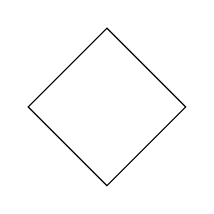
\begin{tikzpicture}
% cartesian coordinates
\coordinate(P) at (1, 3);

% polar coordinates
\coordinate(Q) at (30, 3.5);

% draw lines
\draw (1,0) -- (0,1) -- (-1,0) -- (0,-1) -- cycle;
\end{tikzpicture}

\section{Basic shapes}

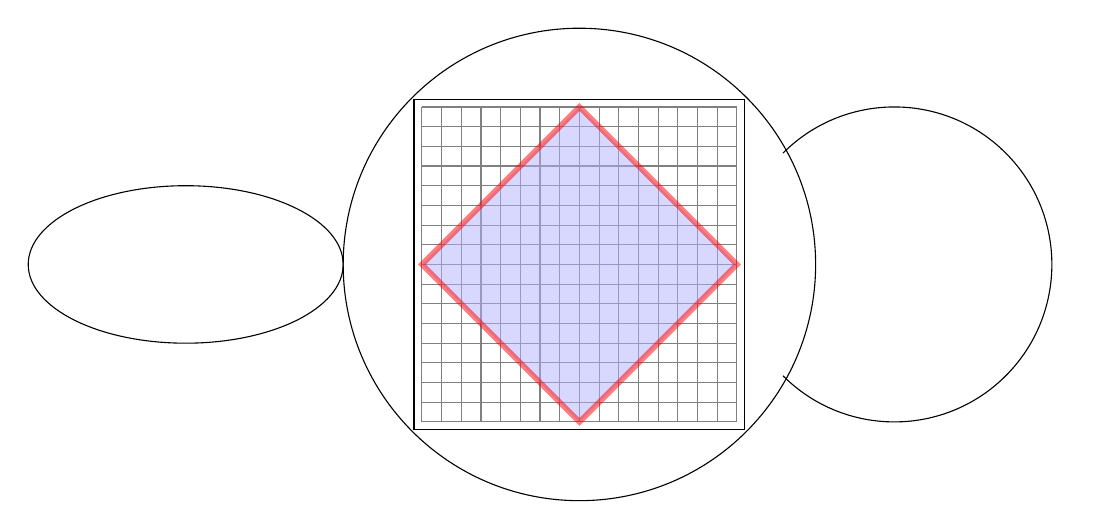
\begin{tikzpicture}
% draw grids from (-2, 2) to (2, 2)
\draw[step=0.25cm,color=gray]
  (-2, -2) grid (2, 2);

\draw[fill,color=blue!30,draw=red,
line width=2pt, opacity=0.5]
  (2,0) -- (0,2) -- (-2,0) -- (0,-2) -- cycle;

% rectangle
\draw (-2.1, -2.1) rectangle (2.1, 2.1);

% circle
\draw (0, 0) circle (3);

% ellipse
\draw (-5, 0) circle (2 and 1);

% arc
\draw (4-1.414, -1.414) arc (-135:135:2);
\end{tikzpicture}

\section{Draw a polygon}

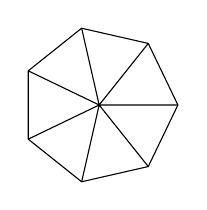
\begin{tikzpicture}
\coordinate (O) at (0, 0);
\coordinate (A) at (360.0/7*0 : 1);
\coordinate (B) at (360.0/7*1 : 1);
\coordinate (C) at (360.0/7*2 : 1);
\coordinate (D) at (360.0/7*3 : 1);
\coordinate (E) at (360.0/7*4 : 1);
\coordinate (F) at (360.0/7*5 : 1);
\coordinate (G) at (360.0/7*6 : 1);

\draw (A) -- (B) -- (C) -- (D) -- (E) -- (F) -- (G) -- cycle;

\draw (O) -- (A)
      (O) -- (B)
      (O) -- (C)
      (O) -- (D)
      (O) -- (E)
      (O) -- (F)
      (O) -- (G);
\end{tikzpicture}

\section{Using loops}

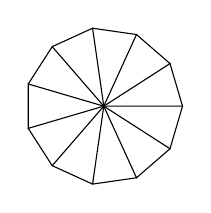
\begin{tikzpicture}
  % for each can be used outside of the tikzpicture
  \foreach \i in {0,...,10}
  {
    \draw (0, 0) -- (360.0/11 * \i : 1)
                 -- ({360.0/11 * (\i + 1)}: 1);
                     % note the curly braces here
  }
\end{tikzpicture}


\section{Nodes}

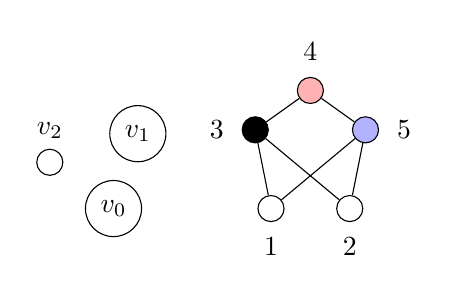
\begin{tikzpicture}

% more examples at
% http://www.texample.net/tikz/examples/feature/node-positioning/
% http://www.texample.net/tikz/examples/bayes/
% http://www.texample.net/tikz/examples/p2p-topology/

\node (v0) at (0, 0) [draw,circle] {$v_0$};
\node (v1) at (1*72 : 1) [draw,circle] {$v_1$};
\node (v2) at (2*72 : 1) [draw,circle,label=$v_2$] {};

% set style here
\tikzstyle{every node}=[draw,shape=circle];
%
\node (r0) at (2, 0) [label=below:1]{};
\node (r1) at (3, 0) [label=below:2]{};
\node (r2) at (1.8, 1) [draw,fill=black,label=left:3]{};
\node (r3) at (3.2, 1) [draw,fill=blue!30,label=right:5]{};
\node (r4) at (2.5, 1.5) [draw,fill=red!30,label=above:4]{};
\draw (r0) -- (r2) (r0) -- (r3) (r1) -- (r2) (r1) -- (r3)
      (r2) -- (r4) (r3) -- (r4);

\end{tikzpicture}



\section{Mathematics operations and functions}

Arithmetic Operators:
\texttt{+ - * / \^}.

Relation Operators:
\texttt{< == >}.

Many function
\texttt{mod, max, min, abs, round, floor,
ceil, exp, ln, pow, sqrt, veclen,
pi, r, rad, deg, sin, cos,
tan, sec, cosec, cot, asin, acos,
atan, rnd, rand}.

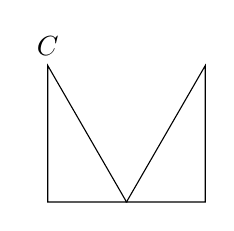
\begin{tikzpicture}
\draw (0,0) -- (1,0) -- (1, {sqrt(3)}) -- cycle;
\coordinate[label=above:$C$] (C) at (-1, {sqrt(3)});
\draw (0,0) -- (-1,0) -- (C) -- cycle;
\end{tikzpicture}

\texttt{\textbackslash usetikzlibrary\{calc\}}


\subsection{Finding midpoints}

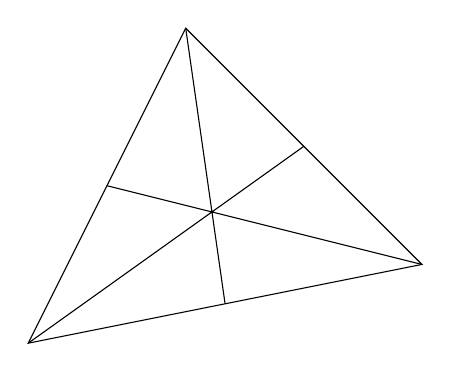
\begin{tikzpicture}
  \coordinate(A) at (0, 0);
  \coordinate(B) at (5, 1);
  \coordinate(C) at (2, 4);
  \coordinate(Ap) at ($(B)!.5!(C)$);
  \coordinate(Bp) at ($(C)!.5!(A)$);
  \coordinate(Cp) at ($(A)!.5!(B)$);

\draw (A) -- (B) -- (C) -- cycle;
\draw (A) -- (Ap) (B) -- (Bp) (C) -- (Cp) ;
\end{tikzpicture}



\subsection{The word \texttt{let}}


\begin{tikzpicture}
\coordinate[label=left:$A$] (A) at (1.2, 2.3);
\coordinate[label=right:$B$] (B) at (3, 4);
\draw (A) -- (B);
\draw (A) let \p1 = ($ (B) - (A) $) in
  circle ({veclen(\x1,\y1)});
\end{tikzpicture}

\subsection{Finding intersections}

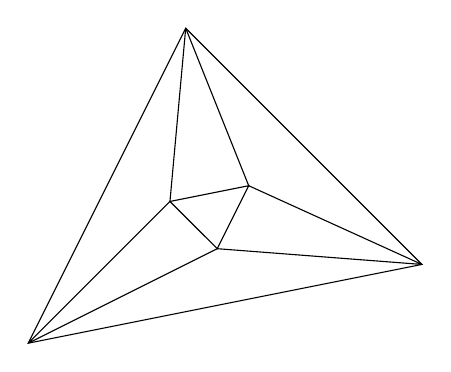
\begin{tikzpicture}
\coordinate(A) at (0, 0);
\coordinate(B) at (5, 1);
\coordinate(C) at (2, 4);
\coordinate(Ap) at ($(B)!1./3!(C)$);
\coordinate(Aq) at ($(B)!2./3!(C)$);
\coordinate(Bp) at ($(C)!1./3!(A)$);
\coordinate(Bq) at ($(C)!2./3!(A)$);
\coordinate(Cp) at ($(A)!1./3!(B)$);
\coordinate(Cq) at ($(A)!2./3!(B)$);

\coordinate (D) at
  (intersection of A--Ap and B--Bq);
\coordinate (E) at
  (intersection of B--Bp and C--Cq);
\coordinate (F) at
  (intersection of C--Cp and A--Aq);

\draw (A) -- (B) -- (C) -- cycle;
\draw (A) -- (D) (B) -- (D)
      (B) -- (E) (C) -- (E)
      (C) -- (F) (A) -- (F);
\draw (D) -- (E) -- (F) -- cycle;
\end{tikzpicture}

\section{In-line PDF output}

Use \texttt{pdflatex}.

\texttt{preview} package.

\tikzstyle{blackdot}=[circle,draw=black,fill=black,
                      inner sep=0pt,minimum size=1mm]
\tikzstyle{whitedot}=[circle,draw=black,fill=white,
                      inner sep=0pt,minimum size=1mm]

We need this
%
\begin{tikzpicture}
  \node (r1) at (0, 0) [whitedot]{};
  \node (r2) at (.3, 0) [whitedot]{};
\node (r3) at (60 : .3) [blackdot]{};
\draw (r1) -- (r2) -- (r3) -- (r1);
\end{tikzpicture}
%
diagram.


This is another inline diagram
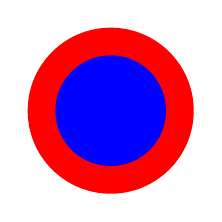
\begin{tikzpicture}
  \fill[red] (0,0) circle (30pt);
  \fill[blue] (0,0) circle (20pt);
\end{tikzpicture}



\section{Automata}

Use the \texttt{automata} and {text}

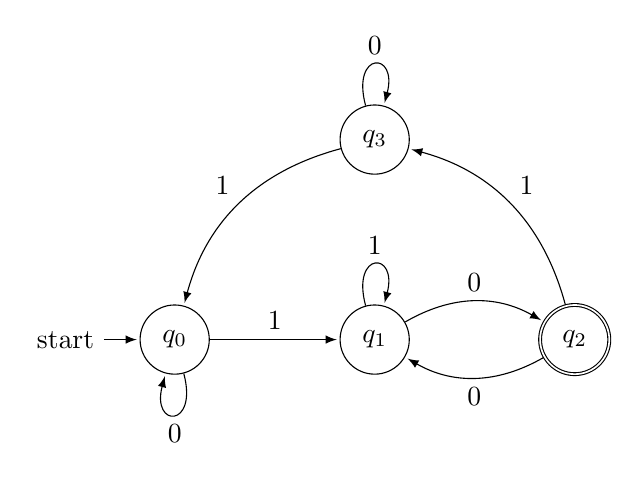
\begin{tikzpicture}[>=latex, shorten >=1pt,
                    node distance=1in, on grid, auto]
% vertices of automaton
\node[state,initial]   (q0)               {$q_0$};
\node[state]           (q1) [right=of q0] {$q_1$};
\node[state,accepting] (q2) [right=of q1] {$q_2$};
\node[state]           (q3) [above=of q1] {$q_3$};

\path[->] (q0) edge [loop below]  node {0} (q0)
          (q0) edge               node {1} (q1)
          (q1) edge [loop above]  node {1} (q1)
          (q1) edge [bend left]   node {0} (q2)
          (q2) edge [bend left]   node {0} (q1)
          (q2) edge [bend right]  node[swap] {1} (q3)
          (q3) edge [bend right]  node[swap] {1} (q0)
          (q3) edge [loop above]  node {0} (q3);

\end{tikzpicture}



\section{Mindmap}

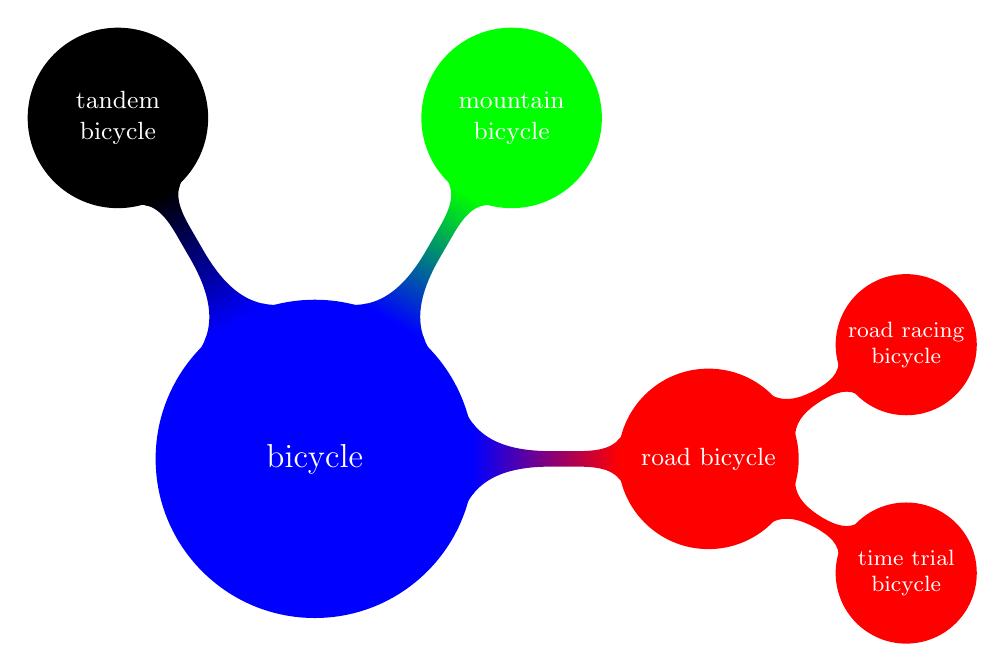
\begin{tikzpicture}
\path[mindmap,concept color=blue,
      text=white,transform shape]
node[concept] {bicycle}
  child[grow=0, concept color=red] {
    node[concept]{road bicycle}
      child[grow=-30] {
        node[concept] {time trial bicycle}
      }
      child[grow=30] {
        node[concept] {road racing bicycle}
      }
  }
  child[grow=60, concept color=green] {
    node[concept]{mountain bicycle}
  }
  child[grow=120, concept color=black] {
    node[concept]{tandem bicycle}
  };
\end{tikzpicture}


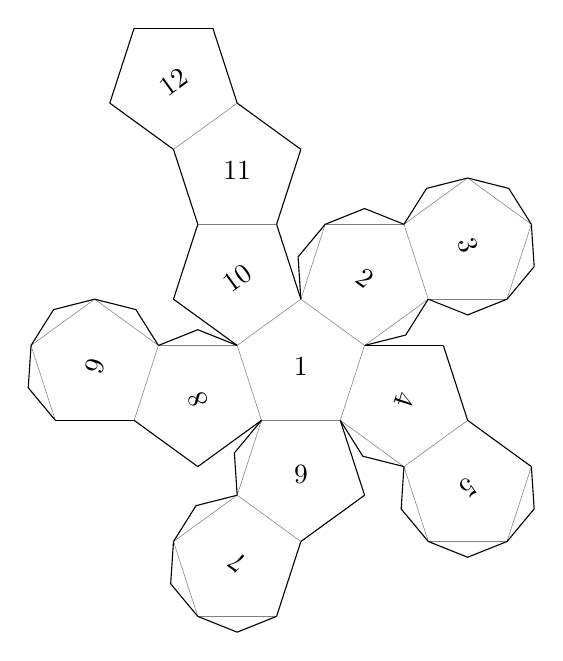
\begin{tikzpicture}[transform shape]
  \tikzfoldingdodecahedron
  [folding line length=10mm,
  face  1 = {\node { 1};},
  face  2 = {\node { 2};},
  face  3 = {\node { 3};},
  face  4 = {\node { 4};},
  face  5 = {\node { 5};},
  face  6 = {\node { 6};},
  face  7 = {\node { 7};},
  face  8 = {\node { 8};},
  face  9 = {\node { 9};},
  face 10 = {\node {10};},
  face 11 = {\node {11};},
  face 12 = {\node {12};}];
\end{tikzpicture}


%\begin{tikzpicture}
%  \draw [help lines, red!50] (0,0) grid (6,4);
%  \draw (0, 0) to [V=V] (0, 4);
%  \draw (0, 4) to (6,4);
%  \draw (1, 4) node[above] {$I \rightarrow$};
%  \draw (6, 4) to [C=C] (6, 0);
%  \draw (4, 4) to [L=L,*-*] (4, 0);
%  \draw (2, 4) to [R=R,*-*] (2, 0);
%  \draw (6, 0) to (0, 0);
%\end{tikzpicture}

\end{document}
